\documentclass[11pt,a4paper,sans]{moderncv}

% moderncv themes
\moderncvtheme[grey]{casual}                 % optional argument are 'blue' (default), 'orange', 'red', 'green', 'grey' and 'roman' (for roman fonts, instead of sans serif fonts)
%\moderncvtheme[green]{casual}                % idem

% character encoding
\usepackage[english,ngerman]{babel}
\usepackage[utf8]{inputenc}                   % replace by the encoding you are using

\usepackage{lmodern}
%\renewcommand{\sfdefault}{\rmdefault}
% adjust the page margins
\usepackage[scale=0.75]{geometry}
\usepackage{graphicx}
%\setlength{\hintscolumnwidth}{3cm}						% if you want to change the width of the column with the dates
%\AtBeginDocument{\setlength{\maketitlenamewidth}{6cm}}  % only for the classic theme, if you want to change the width of your name placeholder (to leave more space for your address details
%\AtBeginDocument{\recomputelengths}                     % required when changes are made to page layout lengths

%----------------------------------------------------------------------------------
%            Kontaktdaten
%----------------------------------------------------------------------------------
% VORNAME
\firstname{lukas}
% NACHNAME
\familyname{elsner}
%TITEL (optional, ggf. einfach die Zeile löschen!)
\title{lebenslauf}
%ADRESSE  (optional, ggf. einfach die Zeile löschen!)
%\address{dorfstrasse 11}{25485 langeln}
%HANDYNUMMER  (optional, ggf. einfach die Zeile löschen!)
%\mobile{0176 20 21 52 67}
%\mobile{(+49) 176 20 21 52 67}
%EMAIL-ADRESSE  (optional, ggf. einfach die Zeile löschen!)
\email{open@mindrunner.de}
%HOMEPAGE  (optional, ggf. einfach die Zeile löschen!)
\homepage{www.mindrunner.de}
%FOTO  (optional, ggf. einfach die Zeile löschen!)
%  64pt = Höhe des Bildes, 'picture' = Name des Bildes
\photo[128pt]{picturesmaller}

% to show numerical labels in the bibliography; only useful if you make citations in your resume
\makeatletter
\renewcommand{\bibliographyitemlabel}{\@biblabel{\arabic{enumiv}}}
\makeatother

%----------------------------------------------------------------------------------
%            Inhalt
%----------------------------------------------------------------------------------

\begin{document}
\maketitle
\section{}
\cvline{geboren}{01.11.1984 in Henstedt-Ulzburg, Deutschland}

\section{ausbildung}
\cventry{2014--2015}{Master of Information Technology}{Queensland University of Technology}{Brisbane}{Australien}{
  \begin{itemize}
    \item Note: 7 / (Entspricht 1,0)
    \item Software Architecture (Advanced)
  \end{itemize}
}
\cventry{2015}{Master Arbeit}{\textbf{[Pyhton, C, Java, VHDL, git, \LaTeX]}}{QUT, Schatz Forensic}{}{
  \begin{itemize}
      \item In diesem Projekt wurde ein low level Framework erstellt, welches
          das Ziel verfolgt Roh-Daten von NAND Speichern, die zum Beispiel
          in SD-Karten und USB-Sticks zu finden sind, auszulesen. Das
          Hardware/Software Co-Design läuft auf einem Pipistrello FPGA Board
          und bietet dynamische Pin-Konfiguration, hohen Datendurchsatz und
          Spannungsanpassung an bestimmten Pins auf der Hardwareseite, sowie
          ein serielles Kommunikationsprotokoll für einen angeschlossenen PC um
          die Hardware zu konfigurieren und Daten auszulesen auf der
          Softwareseite.
  \end{itemize}
}
\cventry{2013--2014}{M.Sc. Informatik}{Universität}{Lübeck}{Master of Science}{
  \begin{itemize}
    \item Software Systems Engineering
  \end{itemize}
}
\cventry{2013}{Software Systems Engineering Praktikum}{\textbf{[Java, Maven,
Jenkins, git \LaTeX]}}{Uni Lübeck}{}{
  \begin{itemize}
     \item Pflichtveranstaltung für jeden Software Systems Engineering Studenten
  \end{itemize}
}
\cventry{2009--2012}{B.Sc. Informatik}{Universität}{Passau}{Bachelor of Science}{
  \begin{itemize}
    \item Note 1,9
    \item Nebenfach Betriebswirtschaftslehre
  \end{itemize}
}
\cventry{2012}{Bachelorarbeit}{\textbf{[C++, \LaTeX]}}{Uni Passau}{\url{http://www.uni-passau.de}}{
  \begin{itemize}
    \item Planung und Implementierung einer einfach zu bedienenden Klassenbibliothek auf Basis eines proprietären SDK um Perzeptionsplattformen zu erstellen mit dem Ziel das Testen im Forschungsprojekt zu automatisieren (Note: 1,3)
  \end{itemize}
}
\cventry{2012}{Wissenschaftliche Hilfskraft}{\textbf{[C++]}}{Uni Passau}{}{
  \begin{itemize}
    \item Umsetzung und Fehlerbehebung in Plugins einer Perzeptionsplatform
    \item Umsetzung von Algorithmen für automatisierte Bild- und Mustererkennung
  \end{itemize}
}
\cventry{2011}{Software Engineering Praktikum}{\textbf{[Java, Maven, Jenkins,
git, \LaTeX]}}{Uni Passau}{}{
  \begin{itemize}
     \item Note 1,0
     \item Pflichtveranstaltung für jeden Informatikstudenten
     \item funCKit ist ein Editor und Simulator für Schaltwerke und Schaltnetze
     \item der Quelltext wurde unter der GPL veröffentlicht\\ (\url{https://github.com/mindrunner/funCKit})
  \end{itemize}
}
\cventry{2005--2008}{Schulische Ausbildung}{Berufsschule}{Elmshorn}{Fachinformatiker}{
  \begin{itemize}
    \item Softwareentwickler
  \end{itemize}
}
\cventry{2005--2008}{Praktische Ausbildung}{TecBOS GmbH}{Halstenbek}{Fachinformatiker}{
  \begin{itemize}
    \item Softwareentwickler
  \end{itemize}
}
\cventry{1995--2004}{Gymnasium}{Dietrich-Bonhoeffer-Gymnasium}{Quickborn}{Abitur}{}

\section{karriere}
\cventry{seit 2004}{Software Engineer / IT-Consultant}{mindrunner}{}{}{
  \begin{itemize}
    \item selbstständige Tätigkeit als Softwareentwickler und Berater
  \end{itemize}
}
\cventry{2010--2011}{Software Engineer}{freifalt GmbH}{Passau/Hamburg}{}{
  \begin{itemize}
    \item Konzeption und Umsetzung von iOS-Apps und deren Backends
    \item verantwortlich für die firmeninterne Infrastruktur, ein virtualisiertes, heterogenes Netzwerk
  \end{itemize}
}
\cventry{2005--2009}{Software Engineer}{MSA Auer GmbH}{Halstenbek/Berlin}{}{
  \begin{itemize}
     \item Entwicklung von diversen Kernprodukten der Firma
  \end{itemize}
}

\section{projekte}

\cventry{2015}{Android Applikation}{\textbf{[Java, Android, Gradle, git-flow, Jira]}}{}{}{
  \begin{itemize}
      \item Entwicklung einer Android App für ein Soziales Netzwerk Startup
      \item Fokussiert auf aktuelle Androit Technologie
    \item REST client / ContentProvider / SyncProvider / Material Design
  \end{itemize}
}
\cventry{2014}{TouchIt}{\textbf{[Java, Android, Gradle, git, libGDX]}}{}{}{
  \begin{itemize}
      \item Entwicklung eines Android Spiels auf Basis von libGDX
      \item Veröffentlicht über den Google Play Store
      \item Source Code veröffentlicht unter GPLv3
    \item \url{https://github.com/mindrunner/touch-it}
  \end{itemize}
}
\cventry{2013--2014}{brightup GmbH}{\textbf{[Java, C, .NET, OpenEmbedded,
git-flow, Jira, Jenkins, BuildBot, Android, iOS]}}{}{http://www.brightup.de}{
  \begin{itemize}
    \item Entwicklung von Hard- und Software für brightups Zentraleinheit und z-wave Steckern
    \item Wartung der Entwicklungstools und Workflows (Bugtracker, Versionsverwaltung, Continuous Integration)
    \item beratende Tätigkeit für Cloud, Smartphone Apps und allgemeinen technischen Entscheidungen
  \end{itemize}
}
\cventry{2013}{PhotoBooth and Quickshot}{\textbf{[Java, Redmine, Jenkins, EDSDK (Canon)]}}{}{}{
  \begin{itemize}
    \item zwei Kiosk-Automat Applikationen für ein Fotostudio
  \end{itemize}
}
\cventry{2013}{hantPlayer}{\textbf{[Objective-C, Remdine, AppKit]}}{}{\url{http://www.hantmade.com}}{
  \begin{itemize}
    \item ein nativer Videoplayer mit speziellen tagging Funktionen
  \end{itemize}
}
\cventry{2013}{Stomt}{\textbf{[Java, MongoDB, Spring, git-flow]}}{}{\url{http://www.stomt.com}}{
  \begin{itemize}
    \item unentgeltliche Arbeit als Berater und Entwickler des Backends und der Android-App
  \end{itemize}
}
\cventry{2012}{HydrostopEU}{\textbf{[Joomla, PHP]}}{}{\url{http://www.hydrostopeu.com}}{
  \begin{itemize}
    \item komplette Überarbeitung der Webseite
  \end{itemize}
}
\cventry{2012}{Nordflair Ticketsystem}{\textbf{[Java, Maven, Jenkins, JPA]}}{}{\url{http://nordflair-events.de/}}{
  \begin{itemize}
    \item Mitentwicklung am Web basiertem Ticket- und Eintrittsmanagementsystem
    \item Entwicklung vom Java-Frontend für das Einlassterminal
  \end{itemize}
}
\cventry{2012}{Templogger}{\textbf{[Java, Maven, Jenkins, JPA]}}{}{}{
  \begin{itemize}
    \item Entwicklung eines Linux Dienstes, der Daten von GSM-Datenloggern entgegen nimmt, in einer Datenbank speichert und bei Überschreiten von Grenzwerten Warn-Emails versendet
  \end{itemize}
}
\cventry{2010--2011}{usAR-Hamburg}{\textbf{[Java, Maven, Jenkins, JPA, iOS]}}{freifalt GmbH}{\url{http://www.freifalt.com}}{
  \begin{itemize}
    \item iOS-App, die auf Basis von Augmented Reality öffentliche Transitmöglichkeiten anzeigt
  \end{itemize}
}
\cventry{2005--2009}{TecBOS.replication}{\textbf{[Delphi]}}{TecBOS GmbH}{\url{http://tecbos.com}}{
  \begin{itemize}
    \item Entwicklung einiger Windows Dienste, mit dem Ziel mehrere TecBOS-Datenbanken zu replizieren
  \end{itemize}
}
\cventry{2005--2009}{TecBOS.mobile}{\textbf{[C, Sqlite]}}{TecBOS GmbH}{\url{http://tecbos.com}}{
  \begin{itemize}
    \item Mobile Windows CE Geräte können mit TecBOS.Solutions Daten austauschen
  \end{itemize}
}
\cventry{2005--2009}{TecBOS.webaccess}{\textbf{[C\#, firebird]}}{TecBOS GmbH}{\url{http://tecbos.com}}{
  \begin{itemize}
    \item Portierung der nativen TecBOS.solutions in eine Web-Applikation
  \end{itemize}
}
\cventry{2005--2009}{TecBOS.solutions}{\textbf{[Delphi, firebird]}}{TecBOS GmbH}{\url{http://tecbos.com}}{
  \begin{itemize}
    \item Entwicklung, Wartung und Pflege der Hauptapplikation
  \end{itemize}
}
\cventry{2008}{CMS}{\textbf{[MySQL, PHP]}}{}{}{
  \begin{itemize}
    \item Entwicklung eines kompletten Content Management Systems innerhalb von einer Woche
  \end{itemize}
}
\cventry{2005--2008}{Webshop}{\textbf{[MySQL, PHP]}}{fontinform GmbH}{\url{http://www.fontinform.com}}{
  \begin{itemize}
    \item Konzeption und Entwicklung eines Webshops für digitale Schriften
  \end{itemize}
}
\section{tech skills}
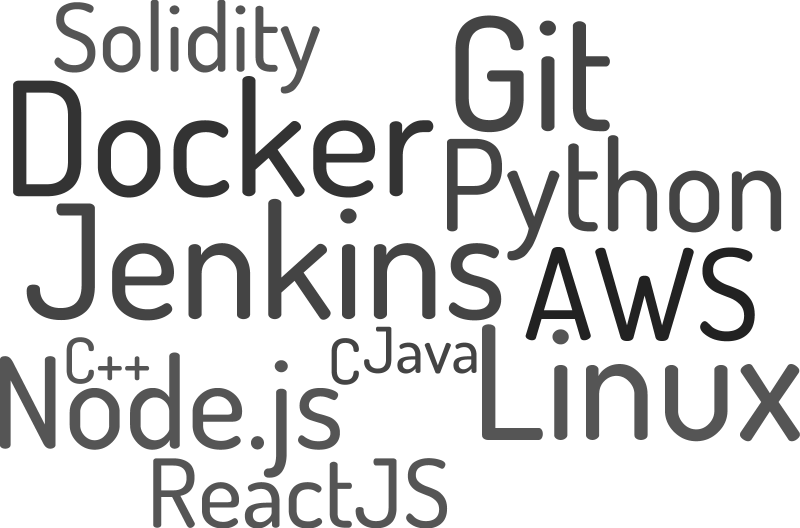
\includegraphics[width=0.7\textwidth]{skillcloud}
%\cvline{Basic}{GTK, Perl, Python, VHDL}{}{}
%\cvline{Advanced}{Android, Bash, C, C++, C\#, Delphi, iOS, Maven, MongoDB, MySQL, PHP}{}{}
%\cvline{Expert}{Debian, Gentoo, Git, OpenEmbedded, Java, \LaTeX, Proxmox, Ubuntu, Yocto}{}{}
%\cvline{Tools}{CMake, Eclipse, Intellij IDE, Make, Netbeans, Vim}{}{}
%\cvline{Miscellaneous}{Office, OS X, Windows}{}{}

\section{sprachen}
\cvline{Deutsch}{Muttersprache}{}
\cvline{Englisch}{Konversationssicher}{}
\cvline{Französisch}{Grundlagen}{}

\section{persönliche interessen}
\cvline{}{\begin{itemize}
    \item klettern
    \item bouldern
    \item laufen
    \item mountainbiken
    \item reisen
\end{itemize}}

~\\
~\\
~\\
Langeln, \today\\ % Aktuelles Datum und Stadt
\end{document}
